\documentclass{acm_proc_article-sp}

\usepackage[brazilian]{babel}
\usepackage[utf8]{inputenc}
\usepackage[T1]{fontenc}

\graphicspath{{figures/}}

\begin{document}
\makeatletter
\def\@copyrightspace{\relax}
\makeatother

\title{Estudo da implementação paralela do quicksort no modelo mestre escravo}

\numberofauthors{2}
\author{
\alignauthor
Diego Pinto da Jornada\\
       \email{pp12804}
\alignauthor
Daniel Antoniazzi Amarante\\
       \email{pp12802}
}

\maketitle
%\begin{abstract}
%Abstract text. Abstract text. Abstract text. Abstract text. Abstract text. Abstract text. Abstract text. 
%\end{abstract}

% A category with the (minimum) three required fields
%\category{H.4}{Information Systems Applications}{Miscellaneous}
%A category including the fourth, optional field follows...
%\category{D.2.8}{Software Engineering}{Metrics}[complexity measures, performance measures]

%\terms{Theory}

%\keywords{ACM proceedings, \LaTeX, text tagging} % NOT required for Proceedings

%TCitation of Einstein paper~\cite{Einstein}.
\section{Introdução}

	No escopo da disciplina de \emph{Programação Paralela} o primeiro 
	trabalho a ser realizado pode ser resumido assim: Analisar o 
	desempenho do algoritmo \emph{quicksort} para ordernar um dada 
	quantidade de vetores, a análise é feita sobre a implementação 
	sequencial e paralela utilizando o modelo mestre escravo.


\section{Modelo da Solução}

	A implementação foi feita de forma que a iniciativa de distrbuição do trabalho é dada através do mestre, ou seja, os escravos não pedem tarefas apenas recebem o trabalho e o no momento em que o mestre recebe uma reposta de algum escravo este escravo. Este modelo apresenta 
	
    

\begin{table}[]
\centering
\caption{Speed-Up data}
\label{my-label}
\begin{tabular}{lllll}
Núcleos & Tempo     & Speed-Up & Eficiência \\
1       & 6.532     & 1,0      & 1,0        \\
2       & 10,629978 & 0,6      & 0,3        \\
4       & 5.67472   & 1,2      & 0,3        \\
8       & 3.989631  & 1,6      & 0,2        \\
16      & 3.593246  & 1,8      & 0,1        \\
32      & 3.781266  & 1,7      & 0,1       
\end{tabular}
\end{table}

\begin{figure}[h]
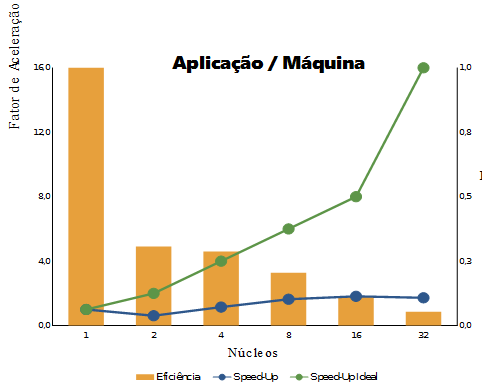
\includegraphics[scale=0.65]{table.png}
\end{figure}

\section{Avaliação do Desempenho}

	Avaliação do desempenho com valores de Speed-Up e eficiência para os casos 
	medidos;


\section{Análise dos Resultado}

	Lorem ipsum dolor sit amet, consectetur adipiscing elit, sed do 
	eiusmod tempor incididunt ut labore et dolore magna aliqua. Ut 
	enim ad minim veniam, quis nostrud exercitation ullamco laboris 
	nisi ut aliquip ex ea commodo consequat. Duis aute irure dolor in 
	reprehenderit in voluptate velit esse cillum dolore eu fugiat 
	nulla pariatur. Excepteur sint occaecat cupidatat non proident, 
	sunt in culpa qui officia deserunt mollit anim id est laborum.

	Lorem ipsum dolor sit amet, consectetur adipiscing elit, sed do 
	eiusmod tempor incididunt ut labore et dolore magna aliqua. Ut 
	enim ad minim veniam, quis nostrud exercitation ullamco laboris 
	nisi ut aliquip ex ea commodo consequat. Duis aute irure dolor in 
	reprehenderit in voluptate velit esse cillum dolore eu fugiat 
	nulla pariatur. Excepteur sint occaecat cupidatat non proident, 
	sunt in culpa qui officia deserunt mollit anim id est laborum.



\section{Dificuldades Encontradas}

	Uma dificuldade encontrada no desenvolvimento do trabalho foi fazer com que o resultado se mantenha ordenado. O mestre deve ter uma maneira de lembrar qual escravo está ordenando o vetor de qual posição, para que quando este for retornado, o mestre possa o colocar na mesma posição de onde ele saiu.



%\bibliographystyle{abbrv}

%\bibliography{sample}

%\balancecolumns 

\end{document}
